%%%%%%%%%%%%%%%%%%%%%%%%%%%%%%%%%%%%%%%%%%%%%%%%%%%%%%%%%%%%%%%%%%%%%%
% Template for a UBC-compliant dissertation
% At the minimum, you will need to change the information found
% after the "Document meta-data"
%
%!TEX TS-program = pdflatex
%!TEX encoding = UTF-8 Unicode

%% The ubcdiss class provides several options:
%%   gpscopy (aka fogscopy)
%%       set parameters to exactly how GPS specifies
%%         * single-sided
%%         * page-numbering starts from title page
%%         * the lists of figures and tables have each entry prefixed
%%           with 'Figure' or 'Table'
%%       This can be tested by `\ifgpscopy ... \else ... \fi'
%%   10pt, 11pt, 12pt
%%       set default font size
%%   oneside, twoside
%%       whether to format for single-sided or double-sided printing
%%   balanced
%%       when double-sided, ensure page content is centred
%%       rather than slightly offset (the default)
%%   singlespacing, onehalfspacing, doublespacing
%%       set default inter-line text spacing; the ubcdiss class
%%       provides \textspacing to revert to this configured spacing
%%   draft
%%       disable more intensive processing, such as including
%%       graphics, etc.
%%


% Commands for editing

\newcommand{\gm}[1]{\textcolor{orange}{{\textit{GM: #1}}}}
\newcommand{\jy}[1]{\textcolor{green}{{\textit{GV: #1}}}}

% For submission to GPS
\documentclass[gpscopy,onehalfspacing,11pt]{ubcdiss}

% Utility commands
\newcommand\printpcnt[2]{\the\numexpr#1*100/#2\%}


% Commands to make reachability questions easier to format
\usepackage{xspace}
\newcommand{\findq}{
  \textit{find SC in TR}\xspace
}
\newcommand{\compareq}{
  \textit{compare($TR_a, TR_b$): $TR_{common}, TR_1, TR_2$}
}

\newcommand{\bsq}[1]{
  \lq{#1}\rq\xspace
}

% For your own copies (looks nicer)
% \documentclass[balanced,twoside,11pt]{ubcdiss}

%%%%%%%%%%%%%%%%%%%%%%%%%%%%%%%%%%%%%%%%%%%%%%%%%%%%%%%%%%%%%%%%%%%%%%
%%%%%%%%%%%%%%%%%%%%%%%%%%%%%%%%%%%%%%%%%%%%%%%%%%%%%%%%%%%%%%%%%%%%%%
%%
%% FONTS:
%% 
%% The defaults below configures Times Roman for the serif font,
%% Helvetica for the sans serif font, and Courier for the
%% typewriter-style font.  Configuring fonts can be time
%% consuming; we recommend skipping to END FONTS!
%% 
%% If you're feeling brave, have lots of time, and wish to use one
%% your platform's native fonts, see the commented out bits below for
%% XeTeX/XeLaTeX.  This is not for the faint at heart. 
%% (And shouldn't you be writing? :-)
%%

%% NFSS font specification (New Font Selection Scheme)
\usepackage{times,mathptmx,courier}
\usepackage[scaled=.92]{helvet}

%% Math or theory people may want to include the handy AMS macros
%\usepackage{amssymb}
\usepackage{amsmath}
\usepackage{icomma}
%\usepackage{amsfonts}

%% The pifont package provides access to the elements in the dingbat font.   
%% Use \ding{##} for a particular dingbat (see p7 of psnfss2e.pdf)
%%   Useful:
%%     51,52 different forms of a checkmark
%%     54,55,56 different forms of a cross (saltyre)
%%     172-181 are 1-10 in open circle (serif)
%%     182-191 are 1-10 black circle (serif)
%%     192-201 are 1-10 in open circle (sans serif)
%%     202-211 are 1-10 in black circle (sans serif)
%% \begin{dinglist}{##}\item... or dingautolist (which auto-increments)
%% to create a bullet list with the provided character.
\usepackage{pifont}

%%%%%%%%%%%%%%%%%%%%%%%%%%%%%%%%%%%%%%%%%%%%%%%%%%%%%%%%%%%%%%%%%%%%%%
%% Configure fonts for XeTeX / XeLaTeX using the fontspec package.
%% Be sure to check out the fontspec documentation.
%\usepackage{fontspec,xltxtra,xunicode}	% required
%\defaultfontfeatures{Mapping=tex-text}	% recommended
%% Minion Pro and Myriad Pro are shipped with some versions of
%% Adobe Reader.  Adobe representatives have commented that these
%% fonts can be used outside of Adobe Reader.
%\setromanfont[Numbers=OldStyle]{Minion Pro}
%\setsansfont[Numbers=OldStyle,Scale=MatchLowercase]{Myriad Pro}
%\setmonofont[Scale=MatchLowercase]{Andale Mono}

%% Other alternatives:
%\setromanfont[Mapping=tex-text]{Adobe Caslon}
%\setsansfont[Scale=MatchLowercase]{Gill Sans}
%\setsansfont[Scale=MatchLowercase,Mapping=tex-text]{Futura}
%\setmonofont[Scale=MatchLowercase]{Andale Mono}
%\newfontfamily{\SYM}[Scale=0.9]{Zapf Dingbats}
%% END FONTS
%%%%%%%%%%%%%%%%%%%%%%%%%%%%%%%%%%%%%%%%%%%%%%%%%%%%%%%%%%%%%%%%%%%%%%
%%%%%%%%%%%%%%%%%%%%%%%%%%%%%%%%%%%%%%%%%%%%%%%%%%%%%%%%%%%%%%%%%%%%%%



%%%%%%%%%%%%%%%%%%%%%%%%%%%%%%%%%%%%%%%%%%%%%%%%%%%%%%%%%%%%%%%%%%%%%%
%%%%%%%%%%%%%%%%%%%%%%%%%%%%%%%%%%%%%%%%%%%%%%%%%%%%%%%%%%%%%%%%%%%%%%
%%
%% Recommended packages
%%
\usepackage{checkend}	% better error messages on left-open environments
\usepackage{graphicx}	% for incorporating external images

%% booktabs: provides some special commands for typesetting tables as used
%% in excellent journals.  Ignore the examples in the Lamport book!
\usepackage{booktabs}

%% listings: useful support for including source code listings, with
%% optional special keyword formatting.  The \lstset{} causes
%% the text to be typeset in a smaller sans serif font, with
%% proportional spacing.
\usepackage{listings}
\lstset{basicstyle=\sffamily\scriptsize,showstringspaces=false,fontadjust}

%% pgfplots: useful support for including visualizations
\usepackage{pgfplots}
\usepackage[caption=false]{subfig}
\usepackage{pgfplotstable}

%% The acronym package provides support for defining acronyms, providing
%% their expansion when first used, and building glossaries.  See the
%% example in glossary.tex and the example usage throughout the example
%% document.
%% NOTE: to use \MakeTextLowercase in the \acsfont command below,
%%   we *must* use the `nohyperlinks' option -- it causes errors with
%%   hyperref otherwise.  See Section 5.2 in the ``LaTeX 2e for Class
%%   and Package Writers Guide'' (clsguide.pdf) for details.
\usepackage[printonlyused,nohyperlinks]{acronym}
%% The ubcdiss.cls loads the `textcase' package which provides commands
%% for upper-casing and lower-casing text.  The following causes
%% the acronym package to typeset acronyms in small-caps
%% as recommended by Bringhurst.
\renewcommand{\acsfont}[1]{{\scshape \MakeTextLowercase{#1}}}

%% color: add support for expressing colour models.  Grey can be used
%% to great effect to emphasize other parts of a graphic or text.
%% For an excellent set of examples, see Tufte's "Visual Display of
%% Quantitative Information" or "Envisioning Information".
\usepackage{color}
\definecolor{greytext}{gray}{0.5}

%% comment: provides a new {comment} environment: all text inside the
%% environment is ignored.
%%   \begin{comment} ignored text ... \end{comment}
\usepackage{comment}

%% The natbib package provides more sophisticated citing commands
%% such as \citeauthor{} to provide the author names of a work,
%% \citet{} to produce an author-and-reference citation,
%% \citep{} to produce a parenthetical citation.
%% We use \citeeg{} to provide examples
\usepackage[numbers,sort&compress]{natbib}
\newcommand{\citeeg}[1]{\citep[e.g.,][]{#1}}

%% The titlesec package provides commands to vary how chapter and
%% section titles are typeset.  The following uses more compact
%% spacings above and below the title.  The titleformat that follow
%% ensure chapter/section titles are set in singlespace.
\usepackage[compact]{titlesec}
\titleformat*{\section}{\singlespacing\raggedright\bfseries\Large}
\titleformat*{\subsection}{\singlespacing\raggedright\bfseries\large}
\titleformat*{\subsubsection}{\singlespacing\raggedright\bfseries}
\titleformat*{\paragraph}{\singlespacing\raggedright\itshape}

%% The caption package provides support for varying how table and
%% figure captions are typeset.
\usepackage[format=hang,indention=-1cm,labelfont={bf},margin=1em]{caption}

%% url: for typesetting URLs and smart(er) hyphenation.
%% \url{http://...} 
\usepackage{url}
\urlstyle{sf}	% typeset urls in sans-serif


%%%%%%%%%%%%%%%%%%%%%%%%%%%%%%%%%%%%%%%%%%%%%%%%%%%%%%%%%%%%%%%%%%%%%%
%%%%%%%%%%%%%%%%%%%%%%%%%%%%%%%%%%%%%%%%%%%%%%%%%%%%%%%%%%%%%%%%%%%%%%
%%
%% Possibly useful packages: you may need to explicitly install
%% these from CTAN if they aren't part of your distribution;
%% teTeX seems to ship with a smaller base than MikTeX and MacTeX.
%%
%\usepackage{pdfpages}	% insert pages from other PDF files
%\usepackage{longtable}	% provide tables spanning multiple pages
%\usepackage{chngpage}	% support changing the page widths on demand
%\usepackage{tabularx}	% an enhanced tabular environment

%% enumitem: support pausing and resuming enumerate environments.
%\usepackage{enumitem}

%% rotating: provides two environments, sidewaystable and sidewaysfigure,
%% for typesetting tables and figures in landscape mode.  
%\usepackage{rotating}

%% subfig: provides for including subfigures within a figure,
%% and includes being able to separately reference the subfigures.
%\usepackage{subfig}

%% ragged2e: provides several new new commands \Centering, \RaggedLeft,
%% \RaggedRight and \justifying and new environments Center, FlushLeft,
%% FlushRight and justify, which set ragged text and are easily
%% configurable to allow hyphenation.
%\usepackage{ragged2e}

%% The ulem package provides a \sout{} for striking out text and
%% \xout for crossing out text.  The normalem and normalbf are
%% necessary as the package messes with the emphasis and bold fonts
%% otherwise.
%\usepackage[normalem,normalbf]{ulem}    % for \sout

%%%%%%%%%%%%%%%%%%%%%%%%%%%%%%%%%%%%%%%%%%%%%%%%%%%%%%%%%%%%%%%%%%%%%%
%% HYPERREF:
%% The hyperref package provides for embedding hyperlinks into your
%% document.  By default the table of contents, references, citations,
%% and footnotes are hyperlinked.
%%
%% Hyperref provides a very handy command for doing cross-references:
%% \autoref{}.  This is similar to \ref{} and \pageref{} except that
%% it automagically puts in the *type* of reference.  For example,
%% referencing a figure's label will put the text `Figure 3.4'.
%% And the text will be hyperlinked to the appropriate place in the
%% document.
%%
%% Generally hyperref should appear after most other packages

%% The `pagebackref' causes the references in the bibliography to have
%% back-references to the citing page; `backref' puts the citing section
%% number.  See further below for other examples of using hyperref.
%% 2009/12/09: now use `linktocpage' (Jacek Kisynski): GPS now prefers
%%   that the ToC, LoF, LoT place the hyperlink on the page number,
%%   rather than the entry text.
\ifgpscopy
  % GPS requires that weblinks should be dark blue, which looks a bit
  % odd in printed form.
  % https://www.grad.ubc.ca/current-students/dissertation-thesis-preparation/fonts-print
  \usepackage[bookmarks,bookmarksnumbered,%
     pagebackref,linktocpage,%
     colorlinks=true,%
     linkcolor=black,%
     urlcolor=blue,%
     citecolor=black%
     ]{hyperref}
\else
  %% The following puts hyperlinks in very faint grey boxes (in pdf only).
  \usepackage[bookmarks,bookmarksnumbered,%
    pagebackref,linktocpage,%
    allbordercolors={0.8 0.8 0.8},%
    ]{hyperref}
\fi
%% The following change how the the back-references text is typeset in a
%% bibliography when `backref' or `pagebackref' are used
%%
%% Change \nocitations if you'd like some text shown where there
%% are no citations found (e.g., pulled in with \nocite{xxx})
\newcommand{\nocitations}{\relax}
%%\newcommand{\nocitations}{No citations}
%%
%\renewcommand*{\backref}[1]{}% necessary for backref < 1.33
\renewcommand*{\backrefsep}{,~}%
\renewcommand*{\backreftwosep}{,~}% ', and~'
\renewcommand*{\backreflastsep}{,~}% ' and~'
\renewcommand*{\backrefalt}[4]{%
\textcolor{greytext}{\ifcase #1%
\nocitations%
\or
\(\rightarrow\) page #2%
\else
\(\rightarrow\) pages #2%
\fi}}


%% The following uses most defaults, which causes hyperlinks to be
%% surrounded by colourful boxes; the colours are only visible in
%% PDFs and don't show up when printed:
%\usepackage[bookmarks,bookmarksnumbered]{hyperref}

%% The following disables the colourful boxes around hyperlinks.
%\usepackage[bookmarks,bookmarksnumbered,pdfborder={0 0 0}]{hyperref}

%% The following disables all hyperlinking, but still enabled use of
%% \autoref{}
%\usepackage[draft]{hyperref}

%% The following commands causes chapter and section references to
%% uppercase the part name.
\renewcommand{\chapterautorefname}{Chapter}
\renewcommand{\sectionautorefname}{Section}
\renewcommand{\subsectionautorefname}{Section}
\renewcommand{\subsubsectionautorefname}{Section}

%% If you have long page numbers (e.g., roman numbers in the 
%% preliminary pages for page 28 = xxviii), you might need to
%% uncomment the following and tweak the \@pnumwidth length
%% (default: 1.55em).  See the tocloft documentation at
%% http://www.ctan.org/tex-archive/macros/latex/contrib/tocloft/
% \makeatletter
% \renewcommand{\@pnumwidth}{3em}
% \makeatother

%%%%%%%%%%%%%%%%%%%%%%%%%%%%%%%%%%%%%%%%%%%%%%%%%%%%%%%%%%%%%%%%%%%%%%
%%%%%%%%%%%%%%%%%%%%%%%%%%%%%%%%%%%%%%%%%%%%%%%%%%%%%%%%%%%%%%%%%%%%%%
%%
%% Some special settings that controls how text is typeset
%%
% \raggedbottom		% pages don't have to line up nicely on the last line
% \sloppy		% be a bit more relaxed in inter-word spacing
% \clubpenalty=10000	% try harder to avoid orphans
% \widowpenalty=10000	% try harder to avoid widows
% \tolerance=1000

%% And include some of our own useful macros
% This file provides examples of some useful macros for typesetting
% dissertations.  None of the macros defined here are necessary beyond
% for the template documentation, so feel free to change, remove, and add
% your own definitions.
%
% We recommend that you define macros to separate the semantics
% of the things you write from how they are presented.  For example,
% you'll see definitions below for a macro \file{}: by using
% \file{} consistently in the text, we can change how filenames
% are typeset simply by changing the definition of \file{} in
% this file.
% 
%% The following is a directive for TeXShop to indicate the main file
%%!TEX root = diss.tex

\newcommand{\NA}{\textsc{n/a}}	% for "not applicable"
\newcommand{\eg}{e.g.,\ }	% proper form of examples (\eg a, b, c)
\newcommand{\ie}{i.e.,\ }	% proper form for that is (\ie a, b, c)
\newcommand{\etal}{\emph{et al}}

% Some useful macros for typesetting terms.
\newcommand{\file}[1]{\texttt{#1}}
\newcommand{\class}[1]{\texttt{#1}}
\newcommand{\latexpackage}[1]{\href{http://www.ctan.org/macros/latex/contrib/#1}{\texttt{#1}}}
\newcommand{\latexmiscpackage}[1]{\href{http://www.ctan.org/macros/latex/contrib/misc/#1.sty}{\texttt{#1}}}
\newcommand{\env}[1]{\texttt{#1}}
\newcommand{\BibTeX}{Bib\TeX}

% Define a command \doi{} to typeset a digital object identifier (DOI).
% Note: if the following definition raise an error, then you likely
% have an ancient version of url.sty.  Either find a more recent version
% (3.1 or later work fine) and simply copy it into this directory,  or
% comment out the following two lines and uncomment the third.
\DeclareUrlCommand\DOI{}
\newcommand{\doi}[1]{\href{http://dx.doi.org/#1}{\DOI{doi:#1}}}
%\newcommand{\doi}[1]{\href{http://dx.doi.org/#1}{doi:#1}}

% Useful macro to reference an online document with a hyperlink
% as well with the URL explicitly listed in a footnote
% #1: the URL
% #2: the anchoring text
\newcommand{\webref}[2]{\href{#1}{#2}\footnote{\url{#1}}}

% epigraph is a nice environment for typesetting quotations
\makeatletter
\newenvironment{epigraph}{%
	\begin{flushright}
	\begin{minipage}{\columnwidth-0.75in}
	\begin{flushright}
	\@ifundefined{singlespacing}{}{\singlespacing}%
    }{
	\end{flushright}
	\end{minipage}
	\end{flushright}}
\makeatother

% \FIXME{} is a useful macro for noting things needing to be changed.
% The following definition will also output a warning to the console
\newcommand{\FIXME}[1]{\typeout{**FIXME** #1}\textbf{[FIXME: #1]}}

% END


%%%%%%%%%%%%%%%%%%%%%%%%%%%%%%%%%%%%%%%%%%%%%%%%%%%%%%%%%%%%%%%%%%%%%%
%%%%%%%%%%%%%%%%%%%%%%%%%%%%%%%%%%%%%%%%%%%%%%%%%%%%%%%%%%%%%%%%%%%%%%
%%
%% Document meta-data: be sure to also change the \hypersetup information
%%

\title{TODO}
\subtitle{TODO}

\author{James Yoo}
\previousdegree{B.Sc., The University of British Columbia, 2020}

% What is this dissertation for?
\degreetitle{Master of Science}

\institution{The University of British Columbia}
\campus{Vancouver}

\faculty{The Faculty of Graduate and Postdoctoral Studies}
\department{Computer Science}
\submissionmonth{TODO}
\submissionyear{2022}

% details of your examining committee
\examiningcommittee{Gail C. Murphy, Professor, Computer Science, UBC}
{Supervisor}
\examiningcommittee{TODO}{Supervisory Committee Member}

%% hyperref package provides support for embedding meta-data in .PDF
%% files
\hypersetup{
  pdftitle={Change this title!  (DRAFT: \today)},
  pdfauthor={Johnny Canuck},
  pdfkeywords={Your keywords here}
}

%%%%%%%%%%%%%%%%%%%%%%%%%%%%%%%%%%%%%%%%%%%%%%%%%%%%%%%%%%%%%%%%%%%%%%
%%%%%%%%%%%%%%%%%%%%%%%%%%%%%%%%%%%%%%%%%%%%%%%%%%%%%%%%%%%%%%%%%%%%%%
%% 
%% The document content
%%

%% LaTeX's \includeonly commands causes any uses of \include{} to only
%% include files that are in the list.  This is helpful to produce
%% subsets of your thesis (e.g., for committee members who want to see
%% the dissertation chapter by chapter).  It also saves time by 
%% avoiding reprocessing the entire file.
%\includeonly{intro,conclusions}
%\includeonly{discussion}

\begin{document}

%%%%%%%%%%%%%%%%%%%%%%%%%%%%%%%%%%%%%%%%%%%%%%%%%%
%% From Thesis Components: Tradtional Thesis
%% <http://www.grad.ubc.ca/current-students/dissertation-thesis-preparation/order-components>

% Preliminary Pages (numbered in lower case Roman numerals)
%    1. Title page (mandatory)
\maketitle

%    2. Committee page (mandatory): lists supervisory committee and,
%    if applicable, the examining committee
\makecommitteepage

%    3. Abstract (mandatory - maximum 350 words)
%% The following is a directive for TeXShop to indicate the main file
%%!TEX root = diss.tex

\chapter{Abstract}

This document provides brief instructions for using the \class{ubcdiss}
class to write a \acs{UBC}-conformant dissertation in \LaTeX.  This
document is itself written using the \class{ubcdiss} class and is
intended to serve as an example of writing a dissertation in \LaTeX.
This document has embedded \acp{URL} and is intended to be viewed
using a computer-based \ac{PDF} reader. Developers write code using software
called an \ac{IDE}.

Note: Abstracts should generally try to avoid using acronyms.

Note: at \ac{UBC}, both the \ac{GPS} Ph.D. defence programme and the
Library's online submission system restricts abstracts to 350
words.

\ifgpscopy
  This document was typeset in \texttt{gpscopy} mode.
\else
  This document was typeset in non-\texttt{gpscopy} mode.
\fi

% Consider placing version information if you circulate multiple drafts
%\vfill
%\begin{center}
%\begin{sf}
%\fbox{Revision: \today}
%\end{sf}
%\end{center}

\cleardoublepage

%    4. Lay Summary (Effective May 2017, mandatory - maximum 150 words)
%% The following is a directive for TeXShop to indicate the main file
%%!TEX root = diss.tex

%% https://www.grad.ubc.ca/current-students/dissertation-thesis-preparation/preliminary-pages
%% 
%% LAY SUMMARY Effective May 2017, all theses and dissertations must
%% include a lay summary.  The lay or public summary explains the key
%% goals and contributions of the research/scholarly work in terms that
%% can be understood by the general public. It must not exceed 150
%% words in length.

\chapter{Lay Summary}

The lay or public summary explains the key goals and contributions of
the research\slash{}scholarly work in terms that can be understood by the
general public. It must not exceed 150 words in length.

\cleardoublepage

%    5. Preface
%% The following is a directive for TeXShop to indicate the main file
%%!TEX root = diss.tex

\chapter{Preface}

All work presented in this thesis was collaboratively conducted in the
Software Practices Laboratory at the University of British Columbia,
Vancouver (Point Grey) campus.

\par I was involved in concept formulation, 
data collection and analysis, and
manuscript composition.
Gail C. Murphy was a supervisory author on this project.
She was involved in all stages of the project, including
concept formulation,
data analysis, and
manuscript composition.

\endinput

TODO: revisit this after collaborating with JetBrains.

\cleardoublepage

%    6. Table of contents (mandatory - list all items in the preliminary pages
%    starting with the abstract, followed by chapter headings and
%    subheadings, bibliographies and appendices)
\tableofcontents
\cleardoublepage	% required by tocloft package

%    7. List of tables (mandatory if thesis has tables)
\listoftables
\cleardoublepage	% required by tocloft package

%    8. List of figures (mandatory if thesis has figures)
\listoffigures
\cleardoublepage	% required by tocloft package

%    9. List of illustrations (mandatory if thesis has illustrations)
%   10. Lists of symbols, abbreviations or other (optional)

%   11. Glossary (optional)
%% The following is a directive for TeXShop to indicate the main file
%%!TEX root = diss.tex

\chapter{Glossary}

This glossary uses the handy \latexpackage{acroynym} package to automatically
maintain the glossary.  It uses the package's \texttt{printonlyused}
option to include only those acronyms explicitly referenced in the
\LaTeX\ source.  To change how the acronyms are rendered, change the
\verb+\acsfont+ definition in \verb+diss.tex+.

% use \acrodef to define an acronym, but no listing
\acrodef{UI}{user interface}
\acrodef{UBC}{University of British Columbia}

% The acronym environment will typeset only those acronyms that were
% *actually used* in the course of the document
\begin{acronym}[ANOVA]
\acro{ANOVA}[ANOVA]{Analysis of Variance\acroextra{, a set of
  statistical techniques to identify sources of variability between groups}}
\acro{CTAN}{\acroextra{The }Common \TeX\ Archive Network}
\acro{EEG}{electroencephalography}
\acro{DOI}{Document Object Identifier\acroextra{ (see
    \url{http://doi.org})}}
\acro{GPS}[GPS]{Graduate and Postdoctoral Studies}
\acro{GUI}[GUI]{Graphical User Interface\acroextra{, a form of user interface
    that enables users to interact with software via visual idioms}}
\acro{UAST}[UAST]{Unified Abstract Syntax Tree\acroextra{,
  a data structure exposed by the IntelliJ IDEA Software Development Kit that 
  enables clients to manipulate program elements in a generalized manner.}}
\acro{API}[API]{Application Programming Interface\acroextra{, a software
    abstraction that enables different software components to communicate with
    one another via a well-defined set of protocols.
}}
\acro{SDK}{Software Development Kit\acroextra{, a collection of related software
    development components that may be used to build for, or extend a specific
    platform.
}}
\acrodefplural{API}[APIs]{Application Programming Interfaces}
\acro{IDE}[IDE]{Integrated Development Environment\acroextra{, a software
    tool for reading, analyzing, and editing source code.}}
\acrodefplural{IDE}[IDE's]{Integrated Development Environments}
\acro{PDF}{Portable Document Format}
\acro{SMT}{Satisfiability Modulo Theories\acroextra{, a generalization
of the classical Boolean satisfiability problem to encompass predicates
from a wider set of theories.}}
\acro{RCS}[RCS]{Revision control system\acroextra{, a software
    tool for tracking changes to a set of files}}
\acro{TLX}[TLX]{Task Load Index\acroextra{, an instrument for gauging
  the subjective mental workload experienced by a human in performing
  a task}}
\acro{UML}{Unified Modelling Language\acroextra{, a visual language
    for modelling the structure of software artefacts}}
\acro{URL}{Unique Resource Locator\acroextra{, used to describe a
    means for obtaining some resource on the world wide web}}
\acro{W3C}[W3C]{\acroextra{the }World Wide Web Consortium\acroextra{,
    the standards body for web technologies}}
\acro{XML}{Extensible Markup Language}
\end{acronym}

% You can also use \newacro{}{} to only define acronyms
% but without explictly creating a glossary
% 
% \newacro{ANOVA}[ANOVA]{Analysis of Variance\acroextra{, a set of
%   statistical techniques to identify sources of variability between groups.}}
% \newacro{API}[API]{application programming interface}
% \newacro{GOMS}[GOMS]{Goals, Operators, Methods, and Selection\acroextra{,
%   a framework for usability analysis.}}
% \newacro{TLX}[TLX]{Task Load Index\acroextra{, an instrument for gauging
%   the subjective mental workload experienced by a human in performing
%   a task.}}
% \newacro{UI}[UI]{user interface}
% \newacro{UML}[UML]{Unified Modelling Language}
% \newacro{W3C}[W3C]{World Wide Web Consortium}
% \newacro{XML}[XML]{Extensible Markup Language}
	% always input, since other macros may rely on it

\textspacing		% begin one-half or double spacing

%   12. Acknowledgements (optional)
%% The following is a directive for TeXShop to indicate the main file
%%!TEX root = diss.tex

\chapter{Acknowledgments}

Thank those people who helped you. 

Don't forget your parents or loved ones.

You may wish to acknowledge your funding sources.


%   13. Dedication (optional)
%% The following is a directive for TeXShop to indicate the main file
%%!TEX root = diss.tex

\chapter{Dedication}
\label{ch:Dedication}

\begin{epigraph}
    \emph{TODO: think about this} 
\end{epigraph}

\endinput



% Body of Thesis (not all sections may apply)
\mainmatter

\acresetall	% reset all acronyms used so far

%    1. Introduction
%% The following is a directive for TeXShop to indicate the main file
%%!TEX root = diss.tex

\chapter{Introduction}
\label{ch:Introduction}

\begin{epigraph}
    \emph{
       A human must turn information into intelligence or knowledge. \\
       We've tended to forget that no computer will ever ask a new question.
     } ---~Rear Admiral Grace M. Hopper
\end{epigraph}

\noindent It has never been easier for software developers to write programs.
There are a plethora of tools that have evolved over the years with the singular
goal of making it easier for developers to write code.
Code-completion tools building on context-dependent analysis 
\cite{reps-1983-context} enable developers to quickly write code in systems they
may not even be familiar with.
Many modern \acp{IDE} are capable of generating
a large amount of boilerplate code at the click of a button.
Recent work in large language models and deep learning \cite{chen-2021-copilot}
has given rise to tools that developers can use to generate entire method 
implementations.
Today, tools are able to present an incredible amount of information, and these 
are only a few in the arsenal of the modern software developer.

\par However, developers engage in a wide variety of tasks;
writing code is only part of their diverse workflows 
\cite{meyer-2017-work-life}.
Developers also analyze requirements and problems, and map out broad flows of
code that may be used to solve a problem.
They also spend a large amount of time attempting to understand code.
This may include activities such as reasoning about the inputs and outputs of
a method, sketching out what the call stack looks like, and even asking 
\emph{why} the code is doing what it is doing \cite{latoza-2006-mental-models}.
A study by Ko et al. found that developers spent approximately 22\% of their
time reading code, while a further 16\% was spent on navigating dependencies.
\cite{ko-2005-eliciting-design}.
This equates to developers spending approximately 38\% of their time on
program comprehension tasks, in comparison to spending approximimately 20\% of
their time on editing code \cite{ko-2005-eliciting-design}.

\par The questions that developers may ask themselves as they attempt to 
understand and modify code are often difficult to answer. 
The difficulty of these questions even appear to be orthogonal to how much
professional experience a developer has, or their familiarity with a codebase
\cite{latoza-2010-reach}.
Questions that developers frequently report as being challenging to answer are
often related to the intent and implementation of code, or associated with 
debugging tasks \cite{latoza-2010-hard-questions}.
To effectively debug their systems and accurately reason about the
intent and implementation of their code, developers often have to trace through
through vast swathes of control-flow paths and filter for task-relevant 
information.
This process of searching through the feasible paths and control-flow of a
program for a set of target statements matching some search criteria can be
formalized as the answering of \emph{reachability questions}
\cite{latoza-2010-reach}.
For example, a developer may ask ``where did some argument \texttt{a} for a 
method \texttt{m} come from?"
This question could be translated to a reachability question that queries the
program for the set of feasible control-flow paths that terminate at the
method \texttt{m}, filtering for statements that include dependencies for
the argument \texttt{a}.

\par Researchers have investigated tools that help developers answer reachability
questions.
tools such as the \emph{Whyline} can help developers reason about
reachability questions by enabling developers to conduct retrospective
debugging sessions of their programs \cite{ko-2004-whyline}.
However, Whyline requires a retrospective program execution trace to generate 
the information needed for a retrospective debugging session. It also limits 
developers to a preset collection of questions-and-answers that they are able to
query.
\emph{GetMeHere} by Microsoft Research attempts to help developers answer
reachability questions by translating them into verification problems that
are dispatched to an \ac{SMT} solver \cite{barnett-2014-get}.
GetMeHere also enables developers to form reachability questions that are more
general in scope, mitigating the limitations associated with constraining
the set of possible reachability questions.
Although the performance of GetMeHere on smaller benchmark programs (e.g.,
650 - $11,000$ LOC) is promising, it has yet to be evaluated on programs that 
are more representative of production software systems today.

% TODO: start on the "in this thesis" section.
% TODO: push this sentence toward the end.

For how far tools have evolved to aid developers in the act of \emph{writing}
code, making the act of \emph{understanding} code easier for developers
appears to be far more challenging.
However, this is not an impossible task.

\endinput

Next steps:
  * Do the "in this thesis" blurb?
  * More background needed?
  * Think about how I can segue into reachability questions.

This document provides a quick set of instructions for using the
\class{ubcdiss} class to write a dissertation in \LaTeX. 
Unfortunately this document cannot provide an introduction to using
\LaTeX.  The classic reference for learning \LaTeX\ is
\citeauthor{lamport-1994-ladps}'s
book~\cite{lamport-1994-ladps}.  There are also many freely-available
tutorials online;
\webref{http://www.andy-roberts.net/misc/latex/}{Andy Roberts' online
    \LaTeX\ tutorials}
seems to be excellent.
The source code for this docment, however, is intended to serve as
an example for creating a \LaTeX\ version of your dissertation.

We start by discussing organizational issues, such as splitting
your dissertation into multiple files, in
\autoref{sec:SuggestedThesisOrganization}.
We then cover the ease of managing cross-references in \LaTeX\ in
\autoref{sec:CrossReferences}.
We cover managing and using bibliographies with \BibTeX\ in
\autoref{sec:BibTeX}. 
We briefly describe typesetting attractive tables in
\autoref{sec:TypesettingTables}.
We briefly describe including external figures in
\autoref{sec:Graphics}, and using special characters and symbols
in \autoref{sec:SpecialSymbols}.
As it is often useful to track different versions of your dissertation,
we discuss revision control further in
\autoref{sec:DissertationRevisionControl}. 
We conclude with pointers to additional sources of information in
\autoref{sec:Conclusions}.

%%%%%%%%%%%%%%%%%%%%%%%%%%%%%%%%%%%%%%%%%%%%%%%%%%%%%%%%%%%%%%%%%%%%%%
\section{Suggested Thesis Organization}
\label{sec:SuggestedThesisOrganization}

The \acs{UBC} \acf{GPS} specifies a particular arrangement of the
components forming a thesis.\footnote{See
    \url{http://www.grad.ubc.ca/current-students/dissertation-thesis-preparation/order-components}}
This template reflects that arrangement.

In terms of writing your thesis, the recommended best practice for
organizing large documents in \LaTeX\ is to place each chapter in
a separate file.  These chapters are then included from the main
file through the use of \verb+\include{file}+.  A thesis might
be described as six files such as \file{intro.tex},
\file{relwork.tex}, \file{model.tex}, \file{eval.tex},
\file{discuss.tex}, and \file{concl.tex}.

We also encourage you to use macros for separating how something
will be typeset (\eg bold, or italics) from the meaning of that
something. 
For example, if you look at \file{intro.tex}, you will see repeated
uses of a macro \verb+\file{}+ to indicate file names.
The \verb+\file{}+ macro is defined in the file \file{macros.tex}.
The consistent use of \verb+\file{}+ throughout the text not only
indicates that the argument to the macro represents a file (providing
meaning or semantics), but also allows easily changing how
file names are typeset simply by changing the definition of the
\verb+\file{}+ macro.
\file{macros.tex} contains other useful macros for properly typesetting
things like the proper uses of the latinate \emph{exempli grati\={a}}
and \emph{id est} (\ie \verb+\eg+ and \verb+\ie+), 
web references with a footnoted \acs{URL} (\verb+\webref{url}{text}+),
as well as definitions specific to this documentation
(\verb+\latexpackage{}+).

%%%%%%%%%%%%%%%%%%%%%%%%%%%%%%%%%%%%%%%%%%%%%%%%%%%%%%%%%%%%%%%%%%%%%%
\section{Making Cross-References}
\label{sec:CrossReferences}

\LaTeX\ make managing cross-references easy, and the \latexpackage{hyperref}
package's\ \verb+\autoref{}+ command\footnote{%
    The \latexpackage{hyperref} package is included by default in this
    template.}
makes it easier still. 

A thing to be cross-referenced, such as a section, figure, or equation,
is \emph{labelled} using a unique, user-provided identifier, defined
using the \verb+\label{}+ command.  
The thing is referenced elsewhere using the \verb+\autoref{}+ command.
For example, this section was defined using:
\begin{lstlisting}
    \section{Making Cross-References}
    \label{sec:CrossReferences}
\end{lstlisting}
References to this section are made as follows:
\begin{lstlisting}
    We then cover the ease of managing cross-references in \LaTeX\
    in \autoref{sec:CrossReferences}.
\end{lstlisting}
\verb+\autoref{}+ takes care of determining the \emph{type} of the 
thing being referenced, so the example above is rendered as
\begin{quote}
    We then cover the ease of managing cross-references in \LaTeX\
    in \autoref{sec:CrossReferences}.
\end{quote}

The label is any simple sequence of characters, numbers, digits,
and some punctuation marks such as ``:'' and ``--''; there should
be no spaces.  Try to use a consistent key format: this simplifies
remembering how to make references.  This document uses a prefix
to indicate the type of the thing being referenced, such as \texttt{sec}
for sections, \texttt{fig} for figures, \texttt{tbl} for tables,
and \texttt{eqn} for equations.

For details on defining the text used to describe the type
of \emph{thing}, search \file{diss.tex} and the \latexpackage{hyperref}
documentation for \texttt{autorefname}.


%%%%%%%%%%%%%%%%%%%%%%%%%%%%%%%%%%%%%%%%%%%%%%%%%%%%%%%%%%%%%%%%%%%%%%
\section{Managing Bibliographies with \BibTeX}
\label{sec:BibTeX}

One of the primary benefits of using \LaTeX\ is its companion program,
\BibTeX, for managing bibliographies and citations.  Managing
bibliographies has three parts: (i) describing references,
(ii)~citing references, and (iii)~formatting cited references.

\subsection{Describing References}

\BibTeX\ defines a standard format for recording details about a
reference.  These references are recorded in a file with a
\file{.bib} extension.  \BibTeX\ supports a broad range of
references, such as books, articles, items in a conference proceedings,
chapters, technical reports, manuals, dissertations, and unpublished
manuscripts. 
A reference may include attributes such as the authors,
the title, the page numbers, the \ac{DOI}, or a \ac{URL}.  A reference
can also be augmented with personal attributes, such as a rating,
notes, or keywords.

Each reference must be described by a unique \emph{key}.\footnote{%
    Note that the citation keys are different from the reference
    identifiers as described in \autoref{sec:CrossReferences}.}
A key is a simple sequence of characters, numbers, digits, and some
punctuation marks such as ``:'' and ``--''; there should be no spaces. 
A consistent key format simiplifies remembering how to make references. 
For example:
\begin{quote}
   \fbox{\emph{last-name}}\texttt{-}\fbox{\emph{year}}\texttt{-}\fbox{\emph{contracted-title}}
\end{quote}
where \emph{last-name} represents the last name for the first author,
and \emph{contracted-title} is some meaningful contraction of the
title.  Then \citeauthor{kiczales-1997-aop}'s seminal article on
aspect-oriented programming~\cite{kiczales-1997-aop} (published in
\citeyear{kiczales-1997-aop}) might be given the key
\texttt{kiczales-1997-aop}.

An example of a \BibTeX\ \file{.bib} file is included as
\file{biblio.bib}.  A description of the format a \file{.bib}
file is beyond the scope of this document.  We instead encourage
you to use one of the several reference managers that support the
\BibTeX\ format such as
\webref{http://jabref.sourceforge.net}{JabRef} (multiple platforms) or
\webref{http://bibdesk.sourceforge.net}{BibDesk} (MacOS\,X only). 
These front ends are similar to reference managers such as
EndNote or RefWorks.


\subsection{Citing References}

Having described some references, we then need to cite them.  We
do this using a form of the \verb+\cite+ command.  For example:
\begin{lstlisting}
    \citet{kiczales-1997-aop} present examples of crosscutting 
    from programs written in several languages.
\end{lstlisting}
When processed, the \verb+\citet+ will cause the paper's authors
and a standardized reference to the paper to be inserted in the
document, and will also include a formatted citation for the paper
in the bibliography.  For example:
\begin{quote}
    \citet{kiczales-1997-aop} present examples of crosscutting 
    from programs written in several languages.
\end{quote}
There are several forms of the \verb+\cite+ command (provided
by the \latexpackage{natbib} package), as demonstrated in
\autoref{tbl:natbib:cite}.
Note that the form of the citation (numeric or author-year) depends
on the bibliography style (described in the next section).
The \verb+\citet+ variant is used when the author names form
an object in the sentence, whereas the \verb+\citep+ variant
is used for parenthetic references, more like an end-note.
Use \verb+\nocite+ to include a citation in the bibliography
but without an actual reference.
\nocite{rowling-1997-hpps}
\begin{table}
\caption{Available \texttt{cite} variants; the exact citation style
    depends on whether the bibliography style is numeric or author-year.}
\label{tbl:natbib:cite}
\centering
\begin{tabular}{lp{3.25in}}\toprule
Variant & Result \\
\midrule
% We cheat here to simulate the cite/citep/citet for APA-like styles
\verb+\cite+ & Parenthetical citation (\eg ``\cite{kiczales-1997-aop}''
    or ``(\citeauthor{kiczales-1997-aop} \citeyear{kiczales-1997-aop})'') \\
\verb+\citet+ & Textual citation: includes author (\eg
    ``\citet{kiczales-1997-aop}'' or
    or ``\citeauthor{kiczales-1997-aop} (\citeyear{kiczales-1997-aop})'') \\
\verb+\citet*+ & Textual citation with unabbreviated author list \\
\verb+\citealt+ & Like \verb+\citet+ but without parentheses \\
\verb+\citep+ & Parenthetical citation (\eg ``\cite{kiczales-1997-aop}''
    or ``(\citeauthor{kiczales-1997-aop} \citeyear{kiczales-1997-aop})'') \\
\verb+\citep*+ & Parenthetical citation with unabbreviated author list \\
\verb+\citealp+ & Like \verb+\citep+ but without parentheses \\
\verb+\citeauthor+ & Author only (\eg ``\citeauthor{kiczales-1997-aop}'') \\
\verb+\citeauthor*+ & Unabbreviated authors list 
    (\eg ``\citeauthor*{kiczales-1997-aop}'') \\
\verb+\citeyear+ & Year of citation (\eg ``\citeyear{kiczales-1997-aop}'') \\
\bottomrule
\end{tabular}
\end{table}

\subsection{Formatting Cited References}

\BibTeX\ separates the citing of a reference from how the cited
reference is formatted for a bibliography, specified with the
\verb+\bibliographystyle+ command. 
There are many varieties, such as \texttt{plainnat}, \texttt{abbrvnat},
\texttt{unsrtnat}, and \texttt{vancouver}.
This document was formatted with \texttt{abbrvnat}.
Look through your \TeX\ distribution for \file{.bst} files. 
Note that use of some \file{.bst} files do not emit all the information
necessary to properly use \verb+\citet{}+, \verb+\citep{}+,
\verb+\citeyear{}+, and \verb+\citeauthor{}+.

There are also packages available to place citations on a per-chapter
basis (\latexpackage{bibunits}), as footnotes (\latexpackage{footbib}),
and inline (\latexpackage{bibentry}).
Those who wish to exert maximum control over their bibliography
style should see the amazing \latexpackage{custom-bib} package.

%%%%%%%%%%%%%%%%%%%%%%%%%%%%%%%%%%%%%%%%%%%%%%%%%%%%%%%%%%%%%%%%%%%%%%
\section{Typesetting Tables}
\label{sec:TypesettingTables}

\citet{lamport-1994-ladps} made one grievous mistake
in \LaTeX: his suggested manner for typesetting tables produces
typographic abominations.  These suggestions have unfortunately
been replicated in most \LaTeX\ tutorials.  These
abominations are easily avoided simply by ignoring his examples
illustrating the use of horizontal and vertical rules (specifically
the use of \verb+\hline+ and \verb+|+) and using the
\latexpackage{booktabs} package instead.

The \latexpackage{booktabs} package helps produce tables in the form
used by most professionally-edited journals through the use of
three new types of dividing lines, or \emph{rules}.
% There are times that you don't want to use \autoref{}
Tables~\ref{tbl:natbib:cite} and~\ref{tbl:LaTeX:Symbols} are two
examples of tables typeset with the \latexpackage{booktabs} package.
The \latexpackage{booktabs} package provides three new commands
for producing rules:
\verb+\toprule+ for the rule to appear at the top of the table,
\verb+\midrule+ for the middle rule following the table header,
and \verb+\bottomrule+ for the bottom-most at the end of the table.
These rules differ by their weight (thickness) and the spacing before
and after.
A table is typeset in the following manner:
\begin{lstlisting}
    \begin{table}
    \caption{The caption for the table}
    \label{tbl:label}
    \centering
    \begin{tabular}{cc}
    \toprule
    Header & Elements \\
    \midrule
    Row 1 & Row 1 \\
    Row 2 & Row 2 \\
    % ... and on and on ...
    Row N & Row N \\
    \bottomrule
    \end{tabular}
    \end{table}
\end{lstlisting}
See the \latexpackage{booktabs} documentation for advice in dealing with
special cases, such as subheading rules, introducing extra space
for divisions, and interior rules.

%%%%%%%%%%%%%%%%%%%%%%%%%%%%%%%%%%%%%%%%%%%%%%%%%%%%%%%%%%%%%%%%%%%%%%
\section{Figures, Graphics, and Special Characters}
\label{sec:Graphics}

Most \LaTeX\ beginners find figures to be one of the more challenging
topics.  In \LaTeX, a figure is a \emph{floating element}, to be
placed where it best fits.
The user is not expected to concern him/herself with the placement
of the figure.  The figure should instead be labelled, and where
the figure is used, the text should use \verb+\autoref+ to reference
the figure's label.
\autoref{fig:latex-affirmation} is an example of a figure.
\begin{figure}
    \centering
    % For the sake of this example, we'll just use text
    %\includegraphics[width=3in]{file}
    \Huge{\textsf{\LaTeX\ Rocks!}}
    \caption{Proof of \LaTeX's amazing abilities}
    \label{fig:latex-affirmation}   % label should change
\end{figure}
A figure is generally included as follows:
\begin{lstlisting}
    \begin{figure}
    \centering
    \includegraphics[width=3in]{file}
    \caption{A useful caption}
    \label{fig:fig-label}   % label should change
    \end{figure}
\end{lstlisting}
There are three items of note:
\begin{enumerate}
\item External files are included using the \verb+\includegraphics+
    command.  This command is defined by the \latexpackage{graphicx} package
    and can often natively import graphics from a variety of formats.
    The set of formats supported depends on your \TeX\ command processor.
    Both \texttt{pdflatex} and \texttt{xelatex}, for example, can
    import \textsc{gif}, \textsc{jpg}, and \textsc{pdf}.  The plain
    version of \texttt{latex} only supports \textsc{eps} files.

\item The \verb+\caption+ provides a caption to the figure. 
    This caption is normally listed in the List of Figures; you
    can provide an alternative caption for the LoF by providing
    an optional argument to the \verb+\caption+ like so:
    \begin{lstlisting}
    \caption[nice shortened caption for LoF]{%
	longer detailed caption used for the figure}
    \end{lstlisting}
    \ac{GPS} generally prefers shortened single-line captions
    in the LoF: multiple-line captions are a bit unwieldy.

\item The \verb+\label+ command provides for associating a unique, user-defined,
    and descriptive identifier to the figure.  The figure can be
    can be referenced elsewhere in the text with this identifier
    as described in \autoref{sec:CrossReferences}.
\end{enumerate}
See Keith Reckdahl’s excellent guide for more details,
\webref{http://www.ctan.org/tex-archive/info/epslatex.pdf}{\emph{Using
imported graphics in LaTeX2e}}.

\section{Special Characters and Symbols}
\label{sec:SpecialSymbols}

\LaTeX\ appropriates many common symbols for its own purposes,
with some used for commands (\eg \verb+\{}&%+) and
mathematics (\eg \verb+$^_+), and others are automagically transformed
into typographically-preferred forms (\eg \verb+-`'+) or to
completely different forms (\eg \verb+<>+).
\autoref{tbl:LaTeX:Symbols} presents a list of common symbols and
their corresponding \LaTeX\ commands.  A much more comprehensive list 
of symbols and accented characters is available at:
\url{http://www.ctan.org/tex-archive/info/symbols/comprehensive/}
\begin{table}
\caption{Useful \LaTeX\ symbols}\label{tbl:LaTeX:Symbols}
\centering\begin{tabular}{ccp{0.5cm}cc}\toprule
\LaTeX & Result && \LaTeX & Result \\
\midrule
    \verb+\texttrademark+ & \texttrademark && \verb+\&+ & \& \\
    \verb+\textcopyright+ & \textcopyright && \verb+\{ \}+ & \{ \} \\
    \verb+\textregistered+ & \textregistered && \verb+\%+ & \% \\
    \verb+\textsection+ & \textsection && \verb+\verb!~!+ & \verb!~! \\
    \verb+\textdagger+ & \textdagger && \verb+\$+ & \$ \\
    \verb+\textdaggerdbl+ & \textdaggerdbl && \verb+\^{}+ & \^{} \\
    \verb+\textless+ & \textless && \verb+\_+ & \_ \\
    \verb+\textgreater+ & \textgreater && \\
\bottomrule
\end{tabular}
\end{table}

%%%%%%%%%%%%%%%%%%%%%%%%%%%%%%%%%%%%%%%%%%%%%%%%%%%%%%%%%%%%%%%%%%%%%%
\section{Changing Page Widths and Heights}

The \class{ubcdiss} class is based on the standard \LaTeX\ \class{book}
class~\cite{lamport-1994-ladps} that selects a line-width to carry
approximately 66~characters per line.  This character density is
claimed to have a pleasing appearance and also supports more rapid
reading~\cite{bringhurst-2002-teots}.  I would recommend that you
not change the line-widths!

\subsection{The \texttt{geometry} Package}

Some students are unfortunately saddled with misguided supervisors
or committee members whom believe that documents should have the
narrowest margins possible.  The \latexpackage{geometry} package is
helpful in such cases.  Using this package is as simple as:
\begin{lstlisting}
    \usepackage[margin=1.25in,top=1.25in,bottom=1.25in]{geometry}
\end{lstlisting}
You should check the package's documentation for more complex uses.

\subsection{Changing Page Layout Values By Hand}

There are some miserable students with requirements for page layouts
that vary throughout the document.  Unfortunately the
\latexpackage{geometry} can only be specified once, in the document's
preamble.  Such miserable students must set \LaTeX's layout parameters
by hand:
\begin{lstlisting}
    \setlength{\topmargin}{-.75in}
    \setlength{\headsep}{0.25in}
    \setlength{\headheight}{15pt}
    \setlength{\textheight}{9in}
    \setlength{\footskip}{0.25in}
    \setlength{\footheight}{15pt}

    % The *sidemargin values are relative to 1in; so the following
    % results in a 0.75 inch margin
    \setlength{\oddsidemargin}{-0.25in}
    \setlength{\evensidemargin}{-0.25in}
    \setlength{\textwidth}{7in}       % 1.1in margins (8.5-2*0.75)
\end{lstlisting}
These settings necessarily require assuming a particular page height
and width; in the above, the setting for \verb+\textwidth+ assumes
a \textsc{US} Letter with an 8.5'' width.
The \latexpackage{geometry} package simply uses the page height and
other specified values to derive the other layout values.
The
\href{http://tug.ctan.org/tex-archive/macros/latex/required/tools/layout.pdf}{\texttt{layout}}
package provides a
handy \verb+\layout+ command to show the current page layout
parameters. 


\subsection{Making Temporary Changes to Page Layout}

There are occasions where it becomes necessary to make temporary
changes to the page width, such as to accomodate a larger formula. 
The \latexmiscpackage{chngpage} package provides an \env{adjustwidth}
environment that does just this.  For example:
\begin{lstlisting}
    % Expand left and right margins by 0.75in
    \begin{adjustwidth}{-0.75in}{-0.75in}
    % Must adjust the perceived column width for LaTeX to get with it.
    \addtolength{\columnwidth}{1.5in}
    \[ an extra long math formula \]
    \end{adjustwidth}
\end{lstlisting}


%%%%%%%%%%%%%%%%%%%%%%%%%%%%%%%%%%%%%%%%%%%%%%%%%%%%%%%%%%%%%%%%%%%%%%
\section{Keeping Track of Versions with Revision Control}
\label{sec:DissertationRevisionControl}

Software engineers have used \acf{RCS} to track changes to their
software systems for decades.  These systems record the changes to
the source code along with context as to why the change was required.
These systems also support examining and reverting to particular
revisions from their system's past.

An \ac{RCS} can be used to keep track of changes to things other
than source code, such as your dissertation.  For example, it can
be useful to know exactly which revision of your dissertation was
sent to a particular committee member.  Or to recover an accidentally
deleted file, or a badly modified image.  With a revision control
system, you can tag or annotate the revision of your dissertation
that was sent to your committee, or when you incorporated changes
from your supervisor.

Unfortunately current revision control packages are not yet targetted
to non-developers.  But the Subversion project's
\webref{http://tortoisesvn.net/docs/release/TortoiseSVN_en/}{TortoiseSVN}
has greatly simplified using the Subversion revision control system
for Windows users.  You should consult your local geek.

A simpler alternative strategy is to create a GoogleMail account
and periodically mail yourself zipped copies of your dissertation.

%%%%%%%%%%%%%%%%%%%%%%%%%%%%%%%%%%%%%%%%%%%%%%%%%%%%%%%%%%%%%%%%%%%%%%
\section{Recommended Packages}

The real strength to \LaTeX\ is found in the myriad of free add-on
packages available for handling special formatting requirements.
In this section we list some helpful packages.

\subsection{Typesetting}

\begin{description}
\item[\latexpackage{enumitem}:]
    Supports pausing and resuming enumerate environments.

\item[\latexpackage{ulem}:]
    Provides two new commands for striking out and crossing out text
    (\verb+\sout{text}+ and \verb+\xout{text}+ respectively)
    The package should likely
    be used as follows:
    \begin{verbatim}
    \usepackage[normalem,normalbf]{ulem}
    \end{verbatim}
    to prevent the package from redefining the emphasis and bold fonts.

\item[\latexpackage{chngpage}:]
    Support changing the page widths on demand.

\item[\latexpackage{mhchem}:] 
    Support for typesetting chemical formulae and reaction equations.

\end{description}

Although not a package, the
\webref{http://www.ctan.org/tex-archive/support/latexdiff/}{\texttt{latexdiff}}
command is very useful for creating changebar'd versions of your
dissertation.


\subsection{Figures, Tables, and Document Extracts}

\begin{description}
\item[\latexpackage{pdfpages}:]
    Insert pages from other PDF files.  Allows referencing the extracted
    pages in the list of figures, adding labels to reference the page
    from elsewhere, and add borders to the pages.

\item[\latexpackage{subfig}:]
    Provides for including subfigures within a figure, and includes
    being able to separately reference the subfigures.  This is a
    replacement for the older \texttt{subfigure} environment.

\item[\latexpackage{rotating}:]
    Provides two environments, sidewaystable and sidewaysfigure,
    for typesetting tables and figures in landscape mode.  

\item[\latexpackage{longtable}:]
    Support for long tables that span multiple pages.

\item[\latexpackage{tabularx}:]
    Provides an enhanced tabular environment with auto-sizing columns.

\item[\latexpackage{ragged2e}:]
    Provides several new commands for setting ragged text (\eg forms
    of centered or flushed text) that can be used in tabular
    environments and that support hyphenation.

\end{description}


\subsection{Bibliography Related Packages}

\begin{description}
\item[\latexpackage{bibunits}:]
    Support having per-chapter bibliographies.

\item[\latexpackage{footbib}:]
    Cause cited works to be rendered using footnotes.

\item[\latexpackage{bibentry}:] 
    Support placing the details of a cited work in-line.

\item[\latexpackage{custom-bib}:]
    Generate a custom style for your bibliography.

\end{description}


%%%%%%%%%%%%%%%%%%%%%%%%%%%%%%%%%%%%%%%%%%%%%%%%%%%%%%%%%%%%%%%%%%%%%%
\section{Moving On}
\label{sec:Conclusions}

At this point, you should be ready to go.  Other handy web resources:
\begin{itemize}
\item \webref{http://www.ctan.org}{\ac{CTAN}} is \emph{the} comprehensive
    archive site for all things related to \TeX\ and \LaTeX. 
    Should you have some particular requirement, somebody else is
    almost certainly to have had the same requirement before you,
    and the solution will be found on \ac{CTAN}.  The links to
    various packages in this document are all to \ac{CTAN}.

\item An online
    \webref{http://www.ctan.org/get/info/latex2e-help-texinfo/latex2e.html}{%
	reference to \LaTeX\ commands} provides a handy quick-reference
    to the standard \LaTeX\ commands.

\item The list of 
    \webref{http://www.tex.ac.uk/cgi-bin/texfaq2html?label=interruptlist}{%
	Frequently Asked Questions about \TeX\ and \LaTeX}
    can save you a huge amount of time in finding solutions to
    common problems.

\item The \webref{http://www.tug.org/tetex/tetex-texmfdist/doc/}{te\TeX\
    documentation guide} features a very handy list of the most useful
    packages for \LaTeX\ as found in \ac{CTAN}.

\item The
\webref{http://www.ctan.org/tex-archive/macros/latex/required/graphics/grfguide.pdf}{\texttt{color}}
    package, part of the graphics bundle, provides handy commands
    for changing text and background colours.  Simply changing
    text to various levels of grey can have a very 
    \textcolor{greytext}{dramatic effect}.


\item If you're really keen, you might want to join the
    \webref{http://www.tug.org}{\TeX\ Users Group}.

\end{itemize}



%    2. Main body
% Generally recommended to put each chapter into a separate file
%% The following is a directive for TeXShop to indicate the main file
%%!TEX root = diss.tex

\chapter{Related Work}
\label{ch:RelatedWork}

\begin{epigraph}
    \emph{
       The computing scientist’s main challenge is not to get confused by the 
       complexities of his own making.
     } ---~Edsger W. Dijkstra
\end{epigraph}

\noindent Researchers have investigated both the questions that developers ask 
as they understand and evolve their systems, and proposed tools that support 
developers in answering their questions during software change tasks.

\par Developers find it challenging to understand code in modern codebases for
a number of reasons.
Many codebases today are large and complex, with some meeting the definition of 
an \emph{ultra-large-scale system} \cite{feiler-2006-ulss}.

\par Google reported in 2016 that its monolithic software codebase was composed
of approximately 1 billion files, with a history of 35 million commits in a
repository that contains 85 terabytes of data and 2 billion lines of code
\cite{potvin-2016-google}.
Of course, not all software systems in existence today are quite comparable in 
scale, but Google's codebase helps to contextualize the challenges that 
developers may face in understanding the systems they wrangle each day.
The size, complexity, and indirection that is becoming commonplace in systems
today \cite{latoza-2010-reach} are pushing the already-elusive goal of
enabling developers to more easily understand their code into new and 
uncharted territories.

\section{Questions that Developers Ask}
\label{sec:QuestionsThatDeveloperAsk}

\noindent Developers have a large number of information needs that must be
addressed during their day-to-day workflows.
These information needs often present themselves as a variety of questions
that require the integration of often-disparate sources of information
\cite{fritz-2010-info-frag}.
For example, to understand how a defect was introduced, a developer may have to
read the source code of a program, find additional context within a bug report
or a project tracker, or resort to speaking to other developers who may have 
more information. 

\par Other questions that developers may ask are more focused, and may involve
querying only one source of information, such as a single program or a
collection of modules in a system.
As developers work to evolve and understand specific parts of their systems,
they may ask: ``where are instances of this class created?" or
``what data can we access from this object?" as they try to discover entities
and relationships in object-oriented systems
\cite{sillito-2006-questions-during-task}.
Additional questions that developers may ask are related to 
the control-flow or the data-flow through a program, such as 
``why isn't control reaching this point in code?" and 
``what parts of this data structure are being accessed in this code?" 
\cite{sillito-2006-questions-during-task}.

\subsection{Reachability Questions}
\label{subsec:ReachabilityQuestions}

\par Researchers have conducted studies that investigate both the 
frequency and difficulty of answering some of the focused questions that 
developers ask during change tasks.
LaToza et al. found that a significant portion of a developer's work involves 
answering reachability questions.
A reachability question is a search across feasible paths through a program for 
target statements matching search criteria \cite{latoza-2010-reach}.
In a survey distributed to 2000 developers employed at Microsoft's Redmond
campus, 460 developers reported asking questions that could be phrased as 
reachability questions more than 9 times a day.
Of the developers who responded, 82\% of them rated one or more of the
reachability questions as at least somewhat hard to answer.
\cite{latoza-2010-reach}.
Not only are reachability questions difficult to answer, but the process of
investigating them is also time-consuming.
A field study of 17 developers found that of the 10 longest activities
undertaken by developers, 9 were associated with reachability questions
\cite{latoza-2010-reach}.

\noindent LaToza et al. formalized two types of reachability questions, named
\textit{find} and \textit{compare} \cite{latoza-2010-reach}.
A \textit{find} question is of the form \findq{}; where \textit{SC} and
\textit{TR} are variable parameters.
\textit{TR} represents a set of concrete program traces, where each trace 
\textit{tr} is a list of tuples $\langle s, env \rangle$. 
In each tuple, $s$ is a statement, and $env$ maps each variable in $s$ to a
value.
\textit{SC} represents search criteria that acts a a function that prunes the
set of traces \textit{TR} to a subset that is relevant to the reachability
question being asked.
As an example of a \textit{find} question, a developer may ask: ``where does
the string \bsq{error} come up in the control-flow of this method called 
\texttt{openConnection}?"
To formalize this into a \textit{find} question, we define \textit{SC} as
$grep(`error\textrm')$, and \textit{TR} as 
$trace(p, \ m_{start}, \ m_{end}, \ C)$, where $p$ is the entire program under
inspection, $m_{start}$ and $m_{end}$ represent the start and end of the
control-flow of the method \texttt{openConnection}, and $C$ is a filtering
constraint that is left unspecified.
The resulting formalization is:
\begin{align*}
  find \ grep(`error\textrm') \ in \ trace(p, \ m_{start}, \ m_{end}, \ C)
\end{align*}
The result of this formalization is a a set of traces that contain statements
where the string \bsq{error} occurs, which a developer may use to help answer
their original question.

\par A \textit{compare} question requires the analysis of two concrete traces, 
and is of the form \compareq{}. 
First, an attempt is made to match each trace $tr_a \in TR_a$ to a trace 
$tr_b \in TR_b$.
The result of this operation may be represented as a list of tuples 
$\langle tr_a, tr_b \rangle$.
For each tuple in the resulting list, \textit{compare} attempts to match 
$\langle s_a, env_a\rangle \in tr_a$ to $\langle s_b, env_b \rangle \in tr_b$.
Each matching tuple is coalesced into traces $tr_{common}$, that form one
of the outputs of the \textit{compare} question: $TR_{common}$.
The tuples in $tr_a$ and $tr_b$ for which no match is found are collected into
the outputs $TR_1$ and $TR_2$, which represent tuples that were found to be 
unique to $TR_a$ and $TR_b$, respectively.
A developer may ask a \textit{compare} question as they refactor code.
``Is this code correct?" \cite{latoza-2010-hard-questions} is a common
question that is often asked.
Assuming ``correct" in the context of refactoring to mean that there are no
functional changes to business logic, the resulting formalization of the
previous question might be:
\begin{align*}
  compare(TR_{pre}, \ TR_{post})
\end{align*}
Where $TR_{pre}$ is the set of traces from the program prior to the refactor,
while $TR_{post}$ is the set of traces from the program after the refactor.
Using $TR_{pre}$ as a ground truth, the developer might inspect the outputs
of the formalization: $T_{common}, T_1,$ and $T_2$, and draw conclusions
regarding the correctness of the refactor.

\section{Answering Reachability Questions}
\label{sec:AnsweringReachabilityQuestions}

\acp{IDE} such as IntelliJ IDEA and Visual Studio include tools that developers 
might adopt in answering reachability questions, even if they were not designed
for that purpose.
For example, a developer might generate a call graph for a set of methods in a
class, and manually traverse it to trace or collect items of interest.
Although a number of built-in tools could be adopted in helping developers
answer reachability questions, it is also suggested that developers could 
perform coding tasks more quickly and accurately with tools that more directly 
support answering reachability questions \cite{latoza-2010-reach}.

\subsection{Low-level Support for Reachability Questions}
\label{subsec:LowLevelSupportReachabilityQuestions}

A common reachability question that developers might ask is: ``where does this
value come from?"
To answer this type of question, a developer could invoke a general-purpose
slicing mechanism (Figure \ref{fig:IntelliJDataflow}) that produces  a set of 
data-flow traces (Figure \ref{fig:IntelliJDataflowResult}).

\par Although the information produced by mechanisms such as general-purpose
slicing and data-flow analysis may be complete and useful, it is difficult
to determine their usability by developers.
The data-flow traces produced by the data-flow analysis tool are presented in a 
very compact view.
This view enables the presentation of a large number of results that does not 
require an equally large amount of visual space.
However, since each row in the output represents a single line of code, it may 
be difficult for developers to understand it with the lack of surrounding
context.
For example, line 200 from Figure \ref{fig:IntelliJDataflowResult} contains the
statement:
\begin{align*}
  % TODO: fix the formatting of this, looks very ugly.
  \texttt{alphaField.document = alphaHexDocument}
\end{align*}
The only information a developer is able to obtain from this statement is that
the \texttt{document} field of the \texttt{alphaField} object was assigned
the value of \texttt{alphaHexDocument}.
It is not possible to obtain more information about the values in the statement
without additional context, which might comprise information useful to 
developers, such as where or how values in a method were assigned, inline 
comments regarding the source code, or even the general structure of the code
that surrounds the statement of interest.

\begin{figure}[ht]
\centering
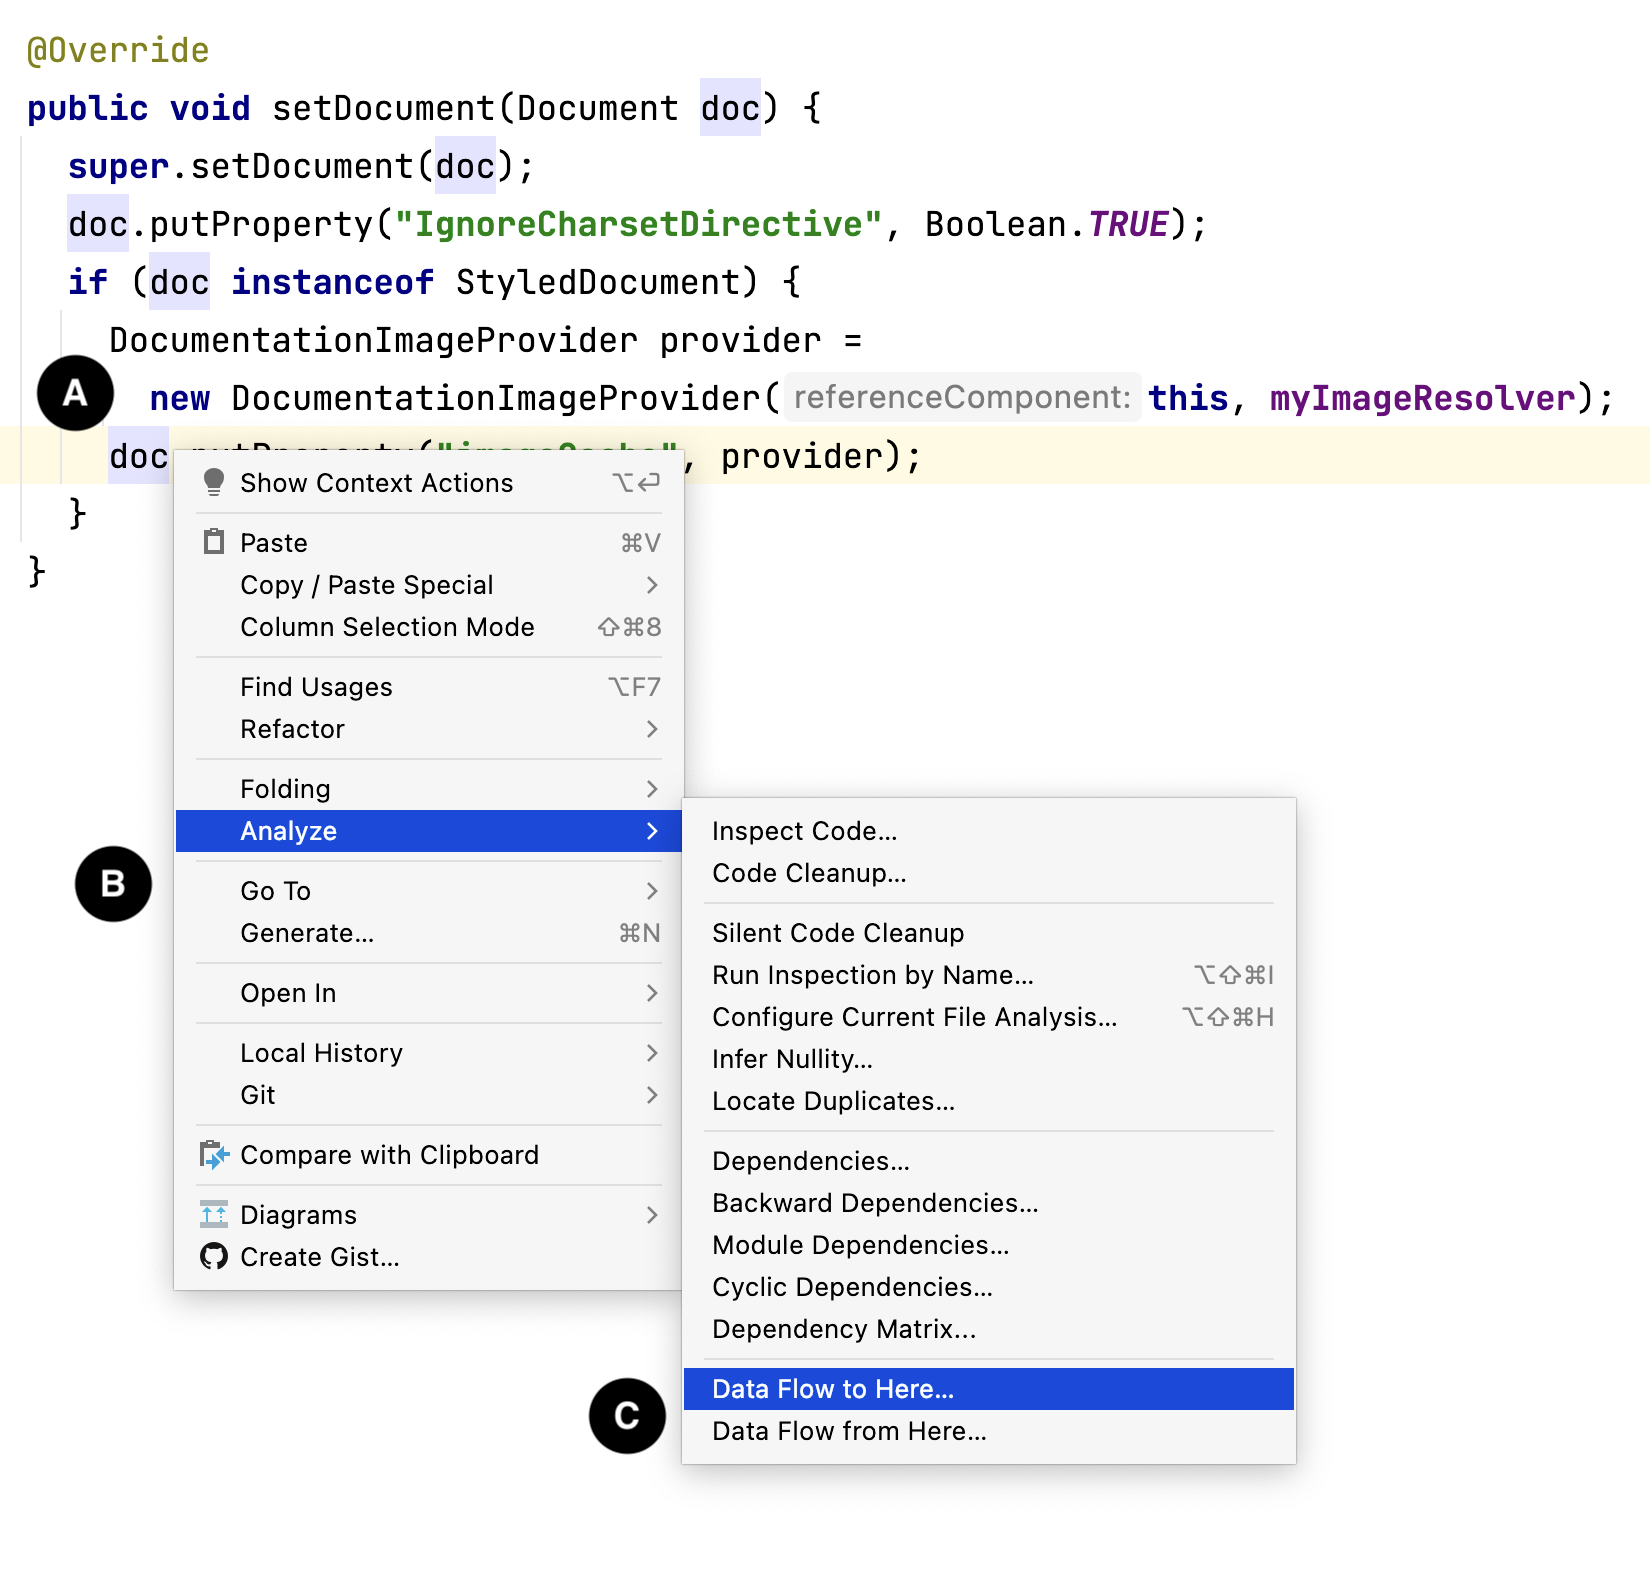
\includegraphics[width=\textwidth]{./figs/intellij-dataflow.png}
\caption{
  A data-flow analysis workflow in IntelliJ IDEA. (A) is the value of
  interest, \texttt{doc}. (B) exposes the variety of analyses that are
  available to developers for \texttt{doc}. (C) invokes a data-flow analysis
  of values that flow into \texttt{doc}.
}
\label{fig:IntelliJDataflow}
\end{figure}

\begin{figure}[ht]
\centering
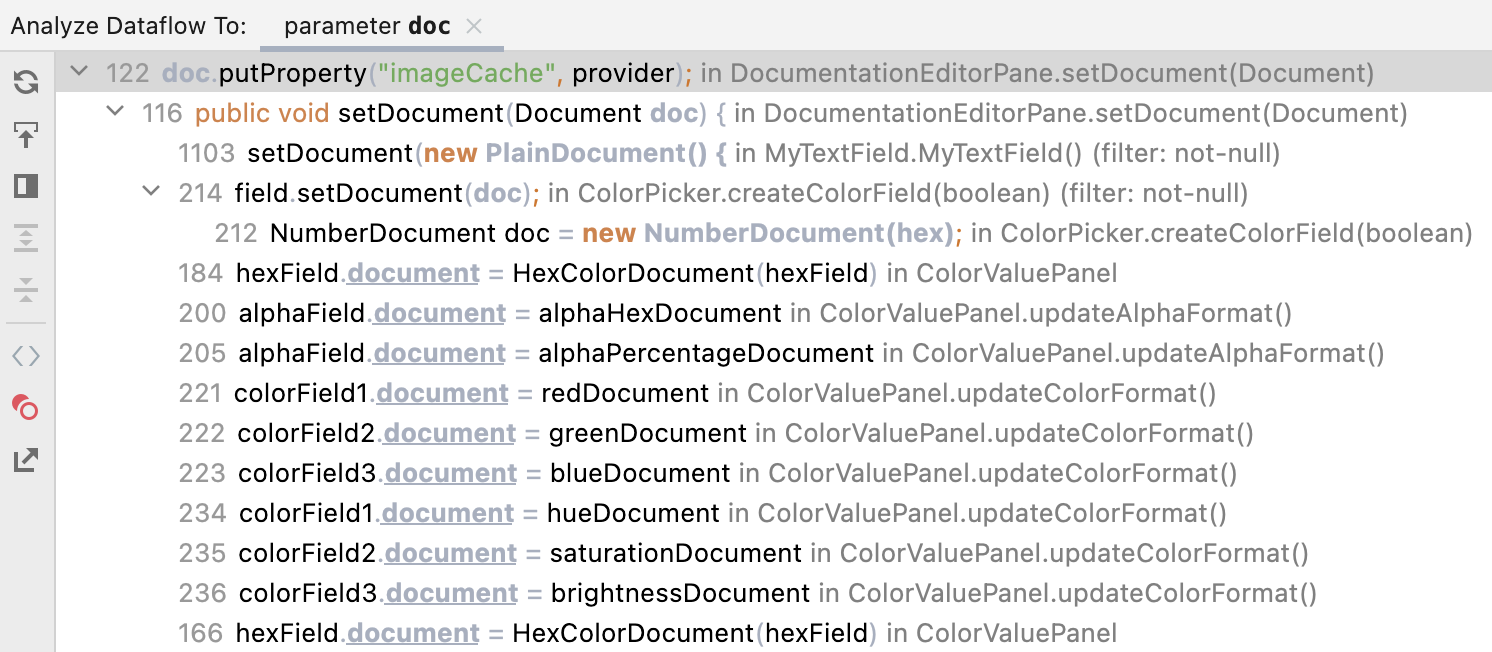
\includegraphics[width=\textwidth]{./figs/intellij-dataflow-result.png}
\caption{
  The output of invoking a ``Dataflow to here..." analysis on \texttt{doc}
  (Figure \ref{fig:IntelliJDataflow}). Each row represents an assignment
  operation to \texttt{doc}. Information such as the line of code, and 
  enclosing method are displayed.
}
\label{fig:IntelliJDataflowResult}
\end{figure}
% TODO: this isn't a question that requires specialized/high-level support

\section{Tools that Support Reachability Questions}
\label{sec:ToolsSupportReachabilityQuestions}

\noindent Tools today employ both dynamic and static approaches to gathering
program information for developers.
For example, the Whyline analyzes runtime information gathered from an offline 
dynamic analysis of an execution trace to generate a set of question and answer 
pairs that are presented to developers \cite{ko-2004-whyline}.
As another example, GetMeHere, developed at Microsoft Research, leverages static 
analysis by translating high-level developer questions into low-level program 
verification problems that are dispatched to an \ac{SMT} solver \cite{barnett-2014-get}, 
removing the need for developers to run their programs to analyze them.

\subsection{The Whyline}
\label{subsec:TheWhyline}

\par The Whyline was initially developed as an interrogative debugging interface
for the Alice programming language. Later, the Java Whyline \cite{ko-2009-java-whyline}
was developed to support the Java programming language and the needs of 
professional developers.
At a high-level, the Whyline enables developers to select questions about a
program's output, and it then helps developers to work back from from the 
selected output to its causes \cite{ko-2009-java-whyline}.
These questions are phrased as ``why did" and ``why didn't"
queries about program output.
For example, consider a case when a variable \texttt{foo} is being erroneously 
set to some value \texttt{v}.
A developer could choose to investigate the cause of this erroneous program
behaviour by running the program, opening the Whyline window and selecting
``why did \texttt{foo} $=$ \texttt{v}?" and a \emph{temporal context}, which is
a specified time-frame that they wish to investigate.
The Whyline then presents a view of all statements of the program within the
temporal context that contributed to the line where \texttt{foo} has the value
\texttt{x}. 
The Whyline's approach of presenting a pre-defined subset of questions about the 
output of programs has benefits, as it avoids speculation about the causes of
a failure, and simplifies the exploration of code responsible for the output
\cite{ko-2009-java-whyline}.
An experiment was conducted to evaluate the efficacy of the Whyline on 
isolating the causes of two bug reports from an open source project \cite{ko-2009-java-whyline}.
It was found that the Whyline users were successful about three times as often
and about twice as fast compared to the control group who used conventional
debugging tools and techniques.

\par Although the Whyline was designed as a stand-alone tool, it presents an 
interface to a developer that resembles those of commonly used \acp{IDE} such
as Microsoft Visual Studio, IntelliJ IDEA, and Eclipse.
Figure \ref{fig:WhylineQuestion} shows the Whyline interface as it is used
to investigate the output of a \ac{GUI} application.
Developers are able to choose a question from the dropdown menu that appears
next to some observable program output.
The Whyline then presents a view that traces the execution of the program
to the specific lines that have an effect on the output under investigation.
This view is presented in Figure \ref{fig:WhylineTrace},
where an editor-like view shows two lines of code in different source files
that affect program output.

\begin{figure}[ht]
\centering
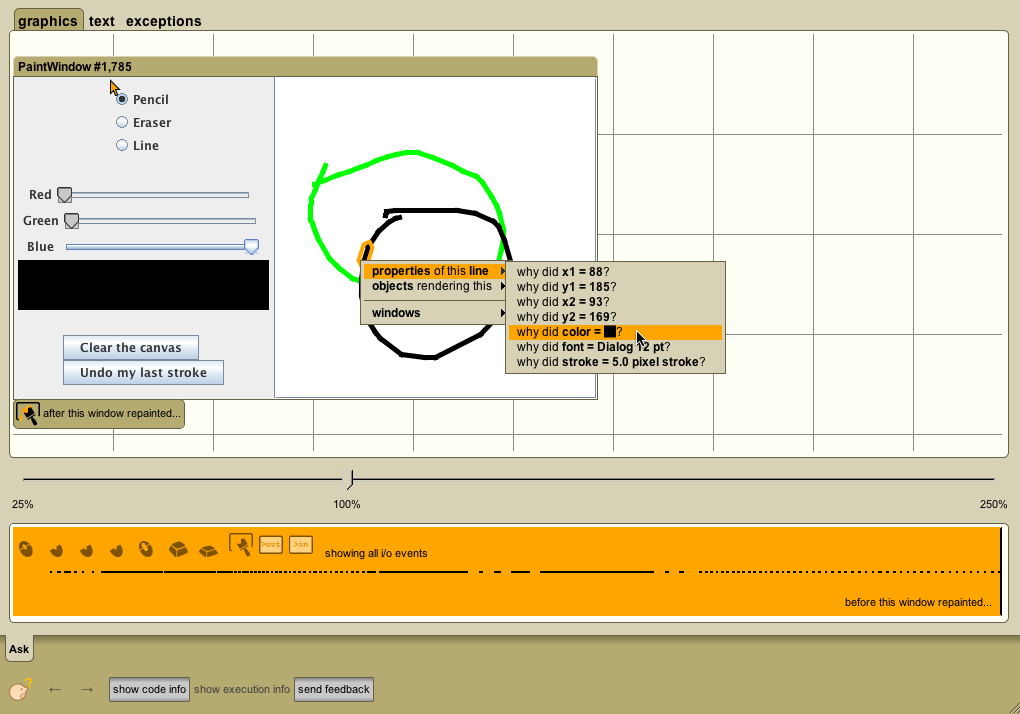
\includegraphics[width=\textwidth]{./figs/whyline-question-interface.png}
\caption{The interrogative debugging interface presented by Whyline.}
\label{fig:WhylineQuestion}
\end{figure}

\begin{figure}[ht]
\centering
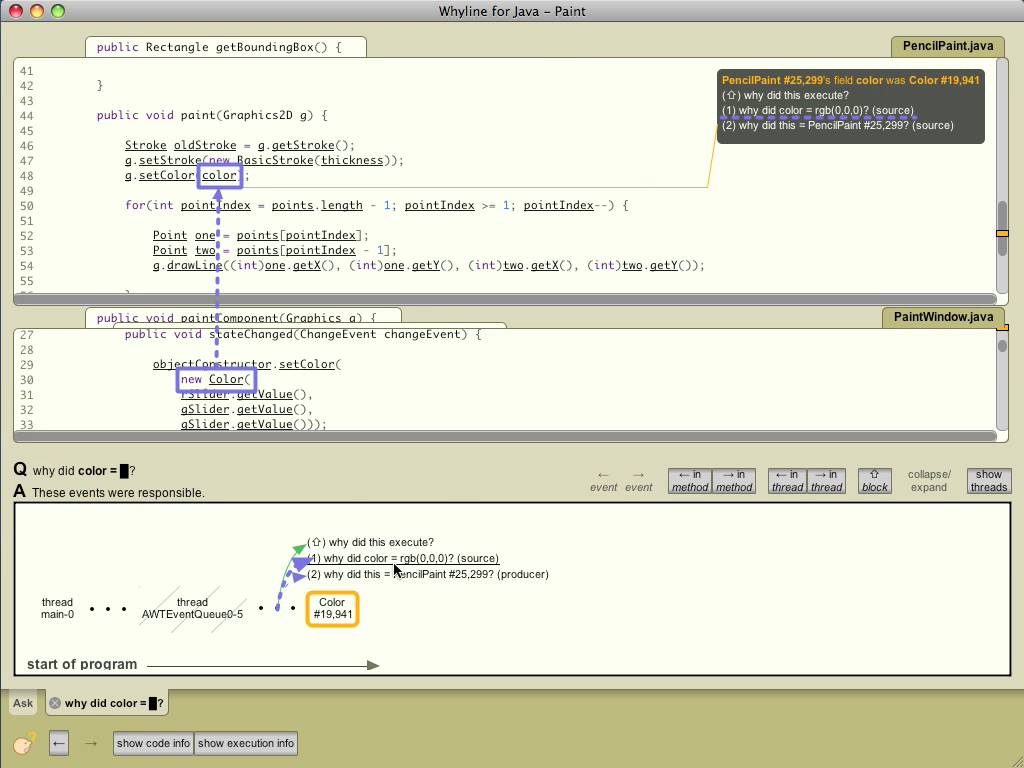
\includegraphics[width=\textwidth]{./figs/whyline-trace-back.png}
\caption{The high-level program trace presented by Whyline.}
\label{fig:WhylineTrace}
\end{figure}

\subsection{GetMeHere}
\label{subsec:GetMeHere}

\par Similar to the Whyline, GetMeHere enables developers to select a line of 
code as a point of interest and visualize the execution that reaches the given 
point.
Where it differs, however, is in how it is able to generate this execution
by using an SMT-based static analysis \cite{barnett-2014-get} without having to
execute the code.
GetMeHere is also presented as a general query engine, where developers can
specify a slice in a program, and execute queries that represent reachability
questions over the given slice \cite{barnett-2014-get}.
The flexibility afforded by GetMeHere enables developers to write queries that 
are highly-parameterizable and specific to the line of investigation they have
chosen to pursue in localizing a defect or understanding a program.
However, with this flexibility comes a danger of enabling program comprehension
or defect localization tasks that may be ultimately unfruitful.
For example, a query that a developer writes to investigate a erroneous value
assignment to a variable might have the possibility of producing results that 
are entirely unrelated to the defect.
The Whyline mitigates these possibilities by presenting a set of questions
and results that are directly formed from an execution trace of a program, and
filtered to include statements and expressions that have dependencies on the
value or object under investigation.
GetMeHere was evaluated on three benchmark programs, all written in C\#.
The sizes of the benchmark programs ranged from 650 to $11,000$ lines of code,
which is relatively small by modern standards.

\par Unlike the Whyline, GetMeHere was built as an extension to the Visual
Studio \ac{IDE}, and not as a standalone application.
GetMeHere displays an execution trace using the Microsoft Debugger Canvas 
\cite{bragdon-2012-canvas}, an industrial implementation of the earlier 
Code Bubbles \cite{bragdon-2010-code-bubbles} paradigm for Visual Studio
\cite{barnett-2014-get}.

\section{How Developers Use Tools to Understand Programs}
\label{sec:HowDevelopersUseToolsToUnderstandPrograms}

\noindent In practice, developers still face difficulties in finding answers 
for their questions during development tasks, even with the tooling available 
to them.
These difficulties appear to be in part due to the inevitability of imperfect 
mappings from high-level developer questions to the low-level analysis 
facilities afforded by program comprehension tools.
In fact, a study of industrial programmers [sic] by Sillito et al. showed that 
participants often struggled to refine and map their questions to tools
that could be used to answer them \cite{sillito-2006-questions-during-task}.

\subsection{Tool Usability}
\label{subsec:ToolUsability}

\par The usability of software engineering tools may also be a significant
factor on how developers use tools to help answer their questions.
Many software tool developers rely on their own intuition for how a tool should
work, eschewing established criteria and procedures for evaluating their 
usability \cite{toleman-98-soft-tools}.
Consequently, the tools available to developers today may be useful, but
ultimately be lacking in terms of their usability.
This lack of usability may even force developers to explore alternative
strategies in understanding and evolving their systems.
In a study of 28 developers from a wide range of companies of different sizes,
Roehm et al. found that 14 of them effectively cloned code due to the
difficulty of understanding the existing code and the consequences of their
changes \cite{roehm-2012-comprehend-software}.
Developers may also choose to abandon the use of purpose-built program
comprehension tools altogether.
In the same study conducted by Roehm et al., 22 developers used an IDE
for development and comprehension tasks.
However, none were observed making use of the IDE's built-in program 
comprehension features, such as visualization and concept localization
\cite{roehm-2012-comprehend-software}.

\subsection{Tool Discovery}
\label{subsec:ToolDiscovery}

Despite the large amount of software tooling available to developers,
it is often the case that they often only use a small subset of the 
commands offered by modern development environments, reducing their overall 
development fluency \cite{murphy-hill-2012-recommend}.
The difficulty in making developers aware of the tools available in their
\acp{IDE} might be related to the general challenge of making end-users aware
of features in software, independent of a specific domain.
For example, a common problem that users faced in a study that examined the
learnability of a software program was that users were not aware of a specific
tool or operation which was available for use \cite{grossman-2009-soft-learn}.

% 
% \par Developers spend a significant portion of the day attempting to answer
% questions about their code.
% Although there are specialized tools that exist to aid developers in this task,
% they are not without their limitations. 
% The Whyline represents a promising approach in enabling developers to answer 
% questions about the runtime behaviour of their code.
% However, it only enables a retrospective analysis of a program, and does not 
% support on-the-fly queries.
% GetMeHere attempts to bypass the need for an execution trace and provide support
% for on-demand queries by translating high-level developer questions into SMT
% instances. 
% Although the results presented by Barnett et al. are promising
% \cite{barnett-2014-get}, the relatively small size of the systems GetMeHere was 
% evaluated on leaves more to be investigated about the scalability of their 
% approach.

\endinput

TODO: add a paragraph about what my thesis attempts to contribute (in relation
to the related work section).


%% The following is a directive for TeXShop to indicate the main file
%%!TEX root = diss.tex

\chapter{Survey}
\label{ch:Survey}

\noindent We deployed a survey to investigate the type and frequency of
reachability questions that developers may encounter during their day-to-day 
activities.

\section{Method}
\label{sec:method}

\noindent The survey was developed with the goal of maximizing the relevance of 
the presented questions to actual scenarios that developers would encounter in
their day-to-day work.
We drew upon our previous work as software developers as well as the literature
for reachability questions \cite{latoza-2010-reach} and hard-to-answer
questions about code that developers ask \cite{latoza-2010-hard-questions}.
From these sources, we drafted a set of 10 questions that we hypothesized 
developers may ask as they performed change tasks or explored their programs.

\par After piloting the survey in a laboratory setting with 7 graduate
students, we finalized a survey with 9 questions with corresponding code
excerpts with a time-to-completion of about 10 minutes.
The survey was deployed entirely online, and consisted of:
\begin{itemize}
    \item 5 demographic questions.
    \item 9 Likert-scale questions that each represented a hypothetical 
          scenario associated with a program comprehension or reachability 
          question.
\end{itemize}

% TODO: describe the survey (use tables?) attach it to this. Make a footnote,

\subsection{Participant Recruitment}
\label{subsec:ParticipantRecruitment}

\noindent
We distributed the survey on Twitter using our personal accounts.
In addition to Twitter, the survey was distributed using mailing lists to
professional software developers.

% TODO: come back to this once we can actually say more about  what we  build
\par As our tool in its current state is targeted toward developers who
use statically-typed programming languages, we excluded respondents who have
never used a statically-typed language as their primary development language.
We also excluded individuals who do not write code at least once a month,
as they may not be the primary audience for an eventual tool.

\section{Survey Results}
\label{sec:SurveyResults}
% TODO: come back after analyzing results.

TODO.

\section{Threats to Validity}
\label{sec:ThreatsToValidity}

% Previously: External Validity

\noindent One of the ways which we distributed our survey was via Twitter.  
This means that part of our results may be specific to the responses of
software developers who use Twitter.
Consequently, it may be challenging to fully generalize our results across
the general population of developers who may not use Twitter.
In an attempt to minimize this threat to validity, we also distributed the 
survey using mailing lists to professional software developers, under the
assumption that most professional software developers use email
\cite{gousios-2016-work-practices}.

% Previously: Construct Validity

\par To create a set of survey questions that would closely represent the
questions and scenarios that developers reported to be most challenging
\cite{latoza-2010-hard-questions, latoza-2010-reach}, we designed a small Java
project represening an e-commerce system.
The Java methods presented in each survey question may not be entirely
representative of the actual code and systems that the respondents may have
experience with.
We deemed this to be an acceptable threat, as the code excerpts we drew from
the sample project were writen to distill the core concepts behind
reachability and program comprehension questions into a succinct representation.
Having overly-complicated code excerpts may have impacted the study by
increasing time-to-completion and drop rate.

\par The code excerpts in our survey were static elements, meaning that the
only way our participants could interact with the code was to read them
in isolation.
Although this furthered our design goal of making the questions encompass
the core concepts behind reachability questions, it did not accurately
capture how developers interact with code (e.g., IDE-based navigation, 
other workflows and tooling) in program comprehension tasks.
To mitigate this threat, we may have had to design our survey around an IDE 
that our participants would be able to use.
However, it is likely that this would have introduced another threat to
validity; our results may be affected by the proficiency of our participants
with the IDE we select to use in our study.
Consequently, we deemed the lack of interactable code excerpts to be an 
acceptable threat.

\par Another threat to validity is the fact that all the code
excerpts included in our survey were written in Java.
This does not account for the fact that our participants may have varying
levels of proficiency with Java.
Consequently, we may be conflating our results with the proficiency of our
participants with Java.
That being said, we needed to select a language for our study that would
have a high likelihood of being familiar to our target audience.
Java's popularity as a development language 
\cite{so-2021-dev-survey, jetbrains-2021-dev-survey} meant that it was a 
suitable choice.

\endinput


%\include{model}
%\include{impl}
%\include{discussion}
%\include{conclusions}

%    3. Notes
%    4. Footnotes

%    5. Bibliography
\begin{singlespace}
\raggedright
\bibliographystyle{abbrvnat}
\bibliography{biblio}
\end{singlespace}

\appendix
%    6. Appendices (including copies of all required UBC Research
%       Ethics Board's Certificates of Approval)
%\include{reb-coa}	% pdfpages is useful here
\chapter{Supporting Materials}

This would be any supporting material not central to the dissertation.
For example:
\begin{itemize}
\item additional details of methodology and/or data;
\item diagrams of specialized equipment developed.;
\item copies of questionnaires and survey instruments.
\end{itemize}


\backmatter
%    7. Index
% See the makeindex package: the following page provides a quick overview
% <http://www.image.ufl.edu/help/latex/latex_indexes.shtml>


\end{document}
